%  Datapath_Design.tex
%  Document created by seblovett on seblovett-Ubuntu
%  Date created: Thu 17 Apr 2014 15:02:16 BST
%  <+Last Edited: Tue 06 May 2014 21:36:15 BST by seblovett on seblovett-Ubuntu +>


\section{Datapath}
\todo[inline, color=green]{MW: Ive done some rewording}

This covers the design of the whole datapath, including circuit diagram.
The datapath consists of arrays of submodules. 
The interrupt constant is also included in the datapath design.
The main submodule is the datapath bit slice. 

%Design of whole module, including circuit diagram
%The datapath consists of arrays of submodules. 
%The interrupt constant is also included in the datapath design.
%The main submodule is the datapath bit slice. 

The program counter, link register, general purpose registers and ALU slices are grouped together into one bitslice.
This module also implements some multiplexors for the Write Data selection and the ALU operand selection.
Other signals are extended to the edges or routed to the relevant locations. 

A ``seventeenth'' slice is also made. 
This includes the three decoders for the registers and the decoder for the ALU.
The register selection multiplexors are implemented in this module as well.
An ALU override was also implemented in this slice.
A series of multiplexors are added to give the controller the ability to conduct an increment / decrement operation. 
This override was added after the initial design to be able to increment the stack pointer irrespective of the current operation.
This was needed to implement the interrupt support to be able to save the Program Counter to the stack.

The final module needed is for the end of the datapath. 
This has the right cell buffer, along with the ALU output register and a tristate buffer.
It also contains an extra tristate buffer to connect the status register (from the controller) to the system bus to allow the storage of the flags.
There are two versions of this module: one to connect an input signal to the system bus, and one to drive the remaining 12 bits of the system bus with a 0. 
This module also contains the memory enable tristate buffer.

\todo[inline]{Circuit diagrams for datapath slice and slice17?}

The full datapath is made up of the following modules:
\begin{enumerate}
\item Datapath Slice
\item Instruction Register modules
\item Left cell buffer
\item LLI cells
\item Right end module
\item Slice seventeen decoders
\end{enumerate}

All blocks are connected in the main datapath module.
The instruction register is routed to the decoders at the top of the module and to the bottom to connect to the controller. 
The system bus outputs and inputs are routed to the right hand side of the module to connect to the pad ring.
Control signals are made available at the bottom of the design to connect to the controller. 

%Design of block,
%The block is constructed as seen in Figure~\ref{fig:datapath:block}
%The tie high and tie low cell are used to set the constant address for the interrupt service routine.
%The instruction register output is routed to both the bottom of the module to be connected to the controller and to the top of the datapath for the decoders and register selects.
%The data in and out connections are routed too the right hand side of the datapath module to make an easy connection to the pad ring. 
%The majority of the control signals are available on the bottom of the datapath, although some, such as the ALU override and register select signals, are only available at the top. 
%This was done so that the controller would sit beneath the datapath and require little routing of the control signals.
%
%\begin{figure}
%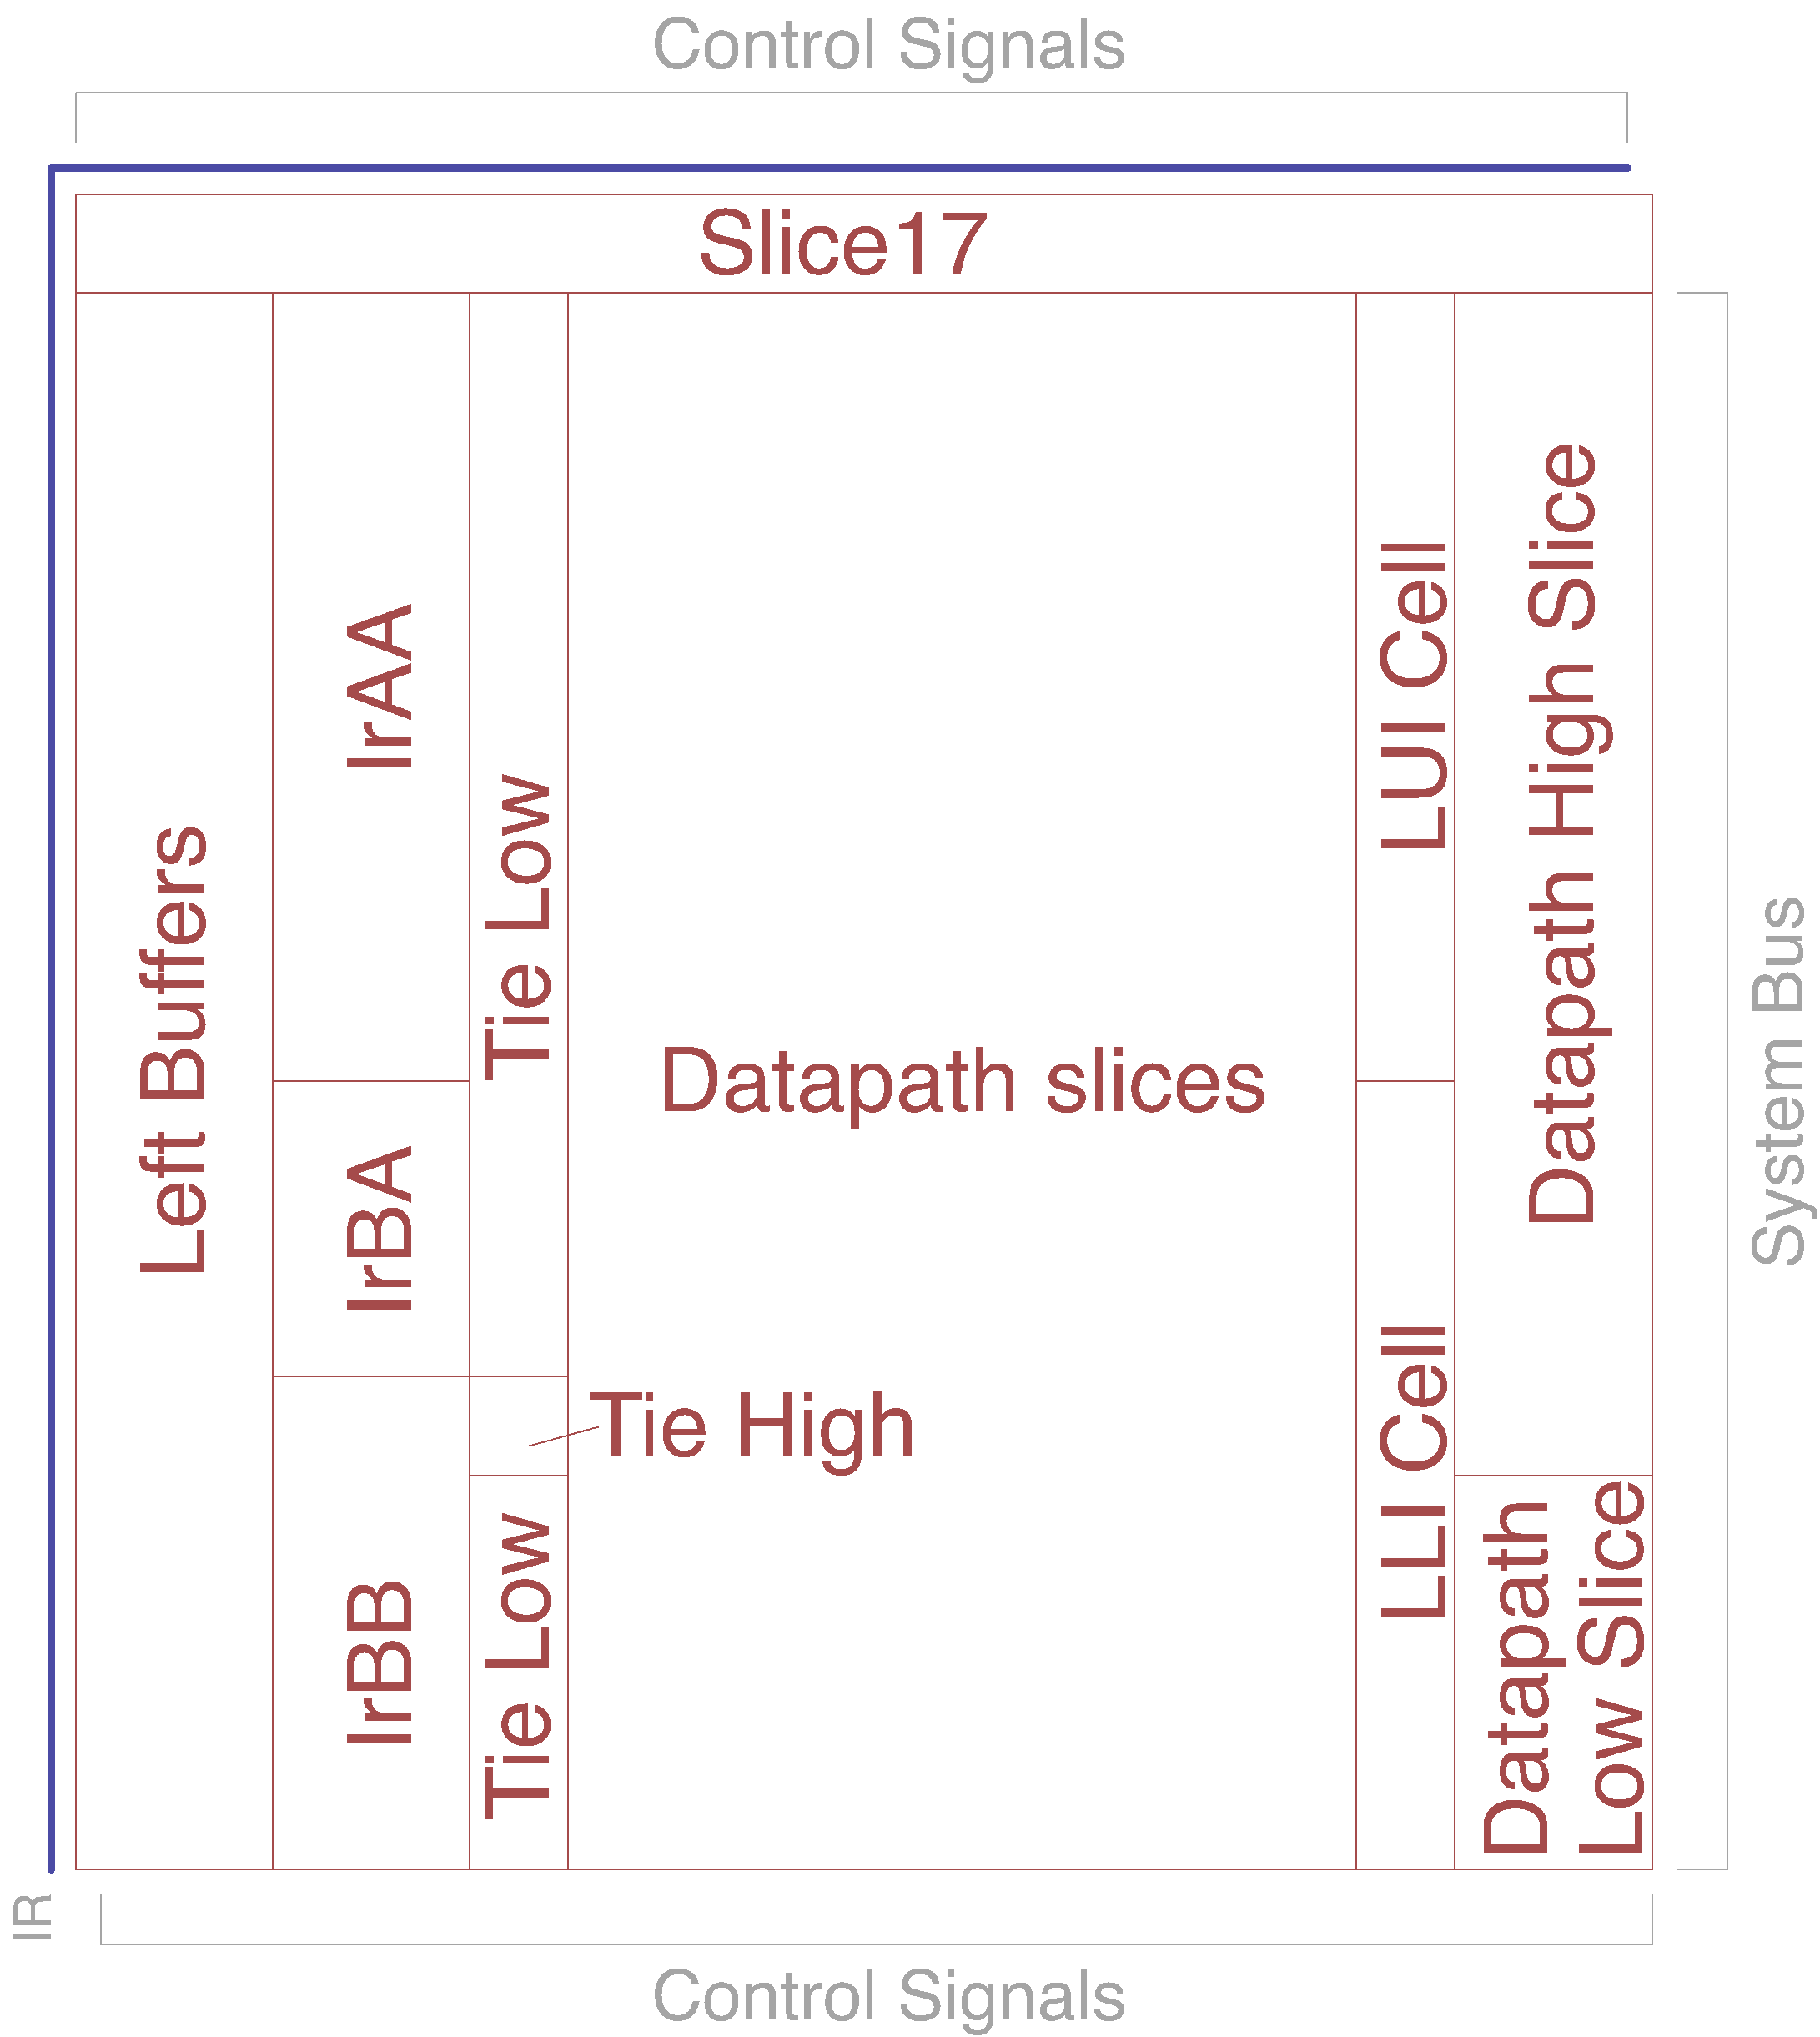
\includegraphics[width=\textwidth]{../../eagle/Datapath/datapath.png}
%\caption{Module layout to make the full datapath.}
%\label{fig:datapath:block}
%\end{figure}

